\documentclass{article}

\usepackage{minted}
\usepackage{amsmath, amsthm}
\usepackage{amssymb}
\usepackage{listings}
\usepackage[svgnames]{xcolor}
\usepackage{tikz}
\usepackage{array}
\usepackage{graphicx}
\usepackage{biblatex}

% Required for Agda
\DeclareUnicodeCharacter{2261}{$\equiv$}
\DeclareUnicodeCharacter{02E1}{${}^1$}
\DeclareUnicodeCharacter{02B3}{${}^r$}
\DeclareUnicodeCharacter{2237}{$::$}
\DeclareUnicodeCharacter{2200}{$\forall$}
\DeclareUnicodeCharacter{220E}{$\blacksquare$}

\usemintedstyle{solarized-light}
\setminted{fontsize=\footnotesize, bgcolor=Beige}

% NOTE: need to run `biber adt_survey` to ensure up-to-date references
\addbibresource{adt_survey.bib}

% TODO CHANGE ALL BUILTINs to BUILT-INs !!!!!!!!!!!!!!!!!!!!!!!!!!!!!!!!!!!!!!!!!!!!!!!!!!!!!!!!!!!!!!!!!!!!!!!!!!!!!!!!!!!!!!!!!!!!!!!!!!!!!!!!!!!!!!!
\title{A Survey on Abstract Data Types}
\author{Anthony Hunt}

\begin{document}
\maketitle
\tableofcontents

\section{Introduction}

From the categorization of species to the periodic table of elements, the organization and manipulation
of data is integral to all aspects of science and technology. Although the collection of data is not a
new field of research by any means, the advent of computerized systems, with its ability to transfer and use
massive amounts of data in mere seconds, necessitates understandable and sensible organization structures.

Over the past 60 years, as computational resource restrictions have eased dramatically,
programming languages and software creation tools have evolved with increasingly better methods of dealing with data.
By viewing pieces of data through specific lenses, programmers can then write algorithms that operate on
any data matching the shape of those lenses, rather than the data itself. These lenses are more commonly referred to as
data types, which assign a type to a piece of data. As we will see later in this paper,
further abstractions over data types themselves enable extremely concise and readable code,
both for the programmer and computer.

The rest of this article will explore data type concepts from 10 languages, % TODO FILL IN
structures to handle errors that might appear, and a small review of ergonomics and usability of those data types.
A necessary discussion of various type systems will naturally evolve as a precursor to data types themselves.

\section{Data Types in 10 Languages} % TODO fill in value for X!!!!!!!!!!!!!!!!!!!!!!!!!!!!!!!!!!!!!!!

Abstract Data Types (ADTs) can look quite different in many languages, but often share the same principles and rules
that make it understandable for programmers. In its essential form, an ADT is a collection of data together with
operations that can be carried out on that data \cite{ADTspec}. The key differences between ADTs from different languages
are the conventions used to collect data and the power operations have over collected data.

In popular object-oriented programming (OOP) languages,
ADTs are approached with a ``class'' mindset, where programmers specify a blueprint for objects that
will eventually be used in a program. For better code reuse, classes can be built from pre-existing classes
through the use of inheritance, a term used to express that a new class inherits all the properties of the old class.
Objects created by classes are referred to as instances of the class and often hold
some amount of mutable data, with methods that have full access to the data. The methods can choose to make use of
``side effects'', referring to the modification of data not explicitly passed through
regular function arguments or return values. Side effects in methods have the consequence that the output of
a method may change independent of the values passed through its arguments. In other words,
the object a method has access to may contain some state that influences the outcome of the method.

At the opposite end of the programming world lies purely functional languages. ADTs in these languages
are more often referred to as data types rather than classes and are only used for collecting and operating on data.
``Objects'' created from these data types are immutable and methods are instead replaced with pure functions that
explicitly take in the relevant data type as input. The operators attached to a functionally pure ADT are functionally
pure themselves, meaning they cannot make use of any hidden state and therefore cannot have side effects.

% Type to express in all languages - a simple linked list, with append and concatenate methods
\subsection{Python}

As a dynamic interpreted scripting language with thousands of high quality libraries and a short learning curve,
Python has become one of the most dominant modern programming languages across several subdomains of computing.
The language itself is characterized mainly by its simple approach to writing readable, practical, and user-friendly code \cite{pythonZen},
used by many as a ``glue'' to easily join high performance computing libraries. The role of Python as a mediator
between optimized C libraries and human understanding, especially in the machine learning space, is adjacent to the role
of documentation in expressing the intention and meaning behind code,
rather than focusing on the small details of the code itself.
% early-age low-level languages and hand-optimized assembly. The abstractions provided from assembly to C,
% and now C to Python, are evident of the trend towards using higher level languages for a better developer experience.
% TODO refer to above comment in the rust section instead

\subsubsection{Python and Types}

The overarching data model behind Python is that everything is either an object or a relation between objects.
Almost all objects in Python are used by reference, and each object contains an identifier (memory address),
an immutable type, and then the actual value itself. In contrast to other scripting languages (namely JavaScript),
an immutable type means that Python will never implicitly recast the type of an object to fit the expected types
of functions or methods (ie. it is strongly typed).

% This behaviour is very different to types in static languages, where names are assigned a type at compile time;
% the runtime objects know their own type and determine which operations can be performed. Thankfully, because of strong
% typing,

Although Python is strongly typed, its lack of a static typing system serves as a double edged sword for
readability and reliability. With small programs, some developers may prefer to just ``get things done'',
making use of whatever combination of built-in types are available.
A mixture of sets, dictionaries, and lists with unrestricted element types are all too common in these types of scripts.
However, assigning proper data types to work with various pieces of information is essential
to the longevity and maintenance of large scale projects. Since the introduction of optional static type hints
via a library in Python 3.5 and increased support through Python 3.8,
a 2022 survey \cite{empiricalTypePython} found a steady increase in the number of GitHub repositories
making use of static type hints.

Aside from granting linters more information to statically analyze the program and warn developers of possible errors,
types also provide programmers themselves with useful information regarding their program. As reinforced
by the philosophy of TypeScript as a type-hinted version of JavaScript, data types serve as an important
channel of communication between programmers. An additional finding of the 2022 survey \cite{empiricalTypePython}
showed that typecheck errors in the linters did not prevent a large amount of code from being pushed, but were
still found to be useful outside of the linter.

Fundamentally, Python places little restriction on the programmer's actions. For example, while
data privacy within Python objects is theoretically possible through name mangled fields (beginning with double-underscores),
there is no real way to completely restrict access to an object's fields so long as that object exists in the code.
Access to deeper implementation details, like a list of current variables, list of fields in any variable, and even
interpreted bytecode is possible through the use of magic methods and variables
(denoted by two underscores at the beginning and end of the identifier).

\subsubsection{Example: A Linked List}

Since Python is primarily an OOP language, the most common form of expressing data types is through the use of classes.
A typical linked list data type in Python 3.11 would look something like:
\inputminted{python}{linked_list/main.py}

Note that Python 3.12 and later make some major changes involving scoping and the syntax of generic types \cite{pythonGenericTypeChange}.

The above \texttt{LinkedList} class expresses the recursive linking nature of the data type while demonstrating
commonly used side effects of OOP methods. Note that the return type for both \texttt{append} and \texttt{concat}
is \texttt{None}. Instead, the data contained within the \texttt{self} object is mutated in place as needed to achieve
the desired functionality.

\subsubsection{Pydantic: A data validation library}

While native Python works well for simple data types like linked lists, type hints do not provide any guarantees
that the type of value, for example, will be consistent across all elements in the list. So, while it does serve as a useful
notation tool for documenting the structure of a data type to other programmers, there are no insurance that the runtime
values for these objects are consistent with the type annotations. As with many topics in Python, a convenient library by the name
of Pydantic will enable both type hints and data validation for those types \textit{at runtime}. The Pydantic version
of our linked list will now look something like:
\inputminted{python}{linked_list/main_pydantic.py}

For this simple data type, only the init function changes. However, under the hood, Pydantic will now ensure that
the type of \texttt{value} within this linked list remains consistent across all elements, throwing an exception
otherwise. Pydantic's version of a class has the ability to transform an OOP construct into one more closely related
to functional programming. If desired, the use of decorators above field names or methods (denoted by \texttt{@decorator})
can restrict mutability, modify constructors, and even change the data validation process to ensure objects are of the correct type.

\subsubsection{Conclusion}

Python's high-level nature, excellent documentation, library support, and exposure of underlying architectures when needed
combine to create a powerful, flexible, and productive language. Although many aspects of the language are initially
hidden or abstracted for the sake of convenience, Python allows programmers to dig deeper into the implementation
when necessary and extend the language in a manner best suited for a specific task.

\subsection{TypeScript}

In JavaScript, types are very loosely bound, and many operations/functions will silently convert types
at runtime. The silent recasting of JavaScript objects combined with unintuitive defaults
can result in very confusing results for the uninitiated. For example, the expression \texttt{1 + "1"}
returns a value of 11 and the expression \texttt{[5, 11, 2].sort()} returns
\texttt{[11, 2, 5]}. In both expressions, the numerical values are converted into strings before the operation is performed.

TypeScript, as an extension of JavaScript with types, is similar to Python in the sense that both
languages started with dynamic typing and patched on static types after the fact, and both aim to resolve issues caused
by dynamic typing. TypeScript (and Python) use types not only for more assurance in program correctness,
but also for the sake of convenience. When making full use of the available typing systems, text editors
and IDEs are able to assist in new code development through intellisense and autocompletion of methods and variables.
Types of objects and documentation for those types additionally appear on mouse-hover, providing fast in-context knowledge.

The below list outlines key properties of types in TypeScript.
\begin{itemize}
    \item Types are treated as sets of values, where types can be part of multiple sets,
    a union of sets, or rarely even an intersection of sets.
    \item Types are structural. Any object containing the required fields needed to be a member of a certain type
    will be considered an object of that type, even if a different type name has been assigned to it.
    Further, if an object has additional fields not specified by the type,
    the extra fields will be ignored in the typechecking process. Essentially, as long as an object meets the minimum
    fields required by the specified type, the object is assumed to be a member of that type.
    \item TypeScript allows any literal string to act as a subset of its respective type,
    with the only allowed value being the literal itself.
    For example, a field with the type \texttt{``name''} will only accept the value of ``name''.
    However, a field with the type \texttt{String} will accept any string object.

\end{itemize}

In comparison to algebraic data types often seen in functional languages, TypeScript replaces inductive data types
with discriminated union sets. For example, our linked list type may look something like:
\inputminted{typescript}{linked_list/main.ts}

Because TypeScript allows literals to act as types, the only valid values in the ``kind'' field
of an object represented by the \texttt{LinkedList} type are our constructor names: ``nil'' or ``cons''.
Although TypeScript treats every object as a reference, similar to Python, we have not used side effects
in the \texttt{append} or \texttt{concat} functions. Instead, we explicitly accept the linked list we want to transform as
input, perform the required action, and return the head of the linked list in the output.

For a non-inductive approach to the LinkedList data type, we can use TypeScript's interfaces to create something that
looks much more like the Pydantic version:
\inputminted{typescript}{linked_list/main_interface.ts}

Finally, a pure OOP version of our LinkedList type, using classes, can be formed.
Note that the append and concat functions are now methods with side effects but are otherwise similar to Python:
\inputminted{typescript}{linked_list/main_class.ts}

\subsection{Rust}

Rust is a unique, high-performance language focused on efficiency and reliability.
While most languages discussed in this paper attempt to either simplify the process of creating software or
formally prove algorithmic correctness, Rust carries a unique blend of practicality and formality.
Among its key features lies a new paradigm of memory management;
rather than using inefficient garbage collectors prominent in almost every OOP language
or dangerous pointers common to imperative C-like languages, Rust introduces the concept of memory ownership.
If safe Rust code is able to pass successfully through the compiler,
it is near-impossible to create memory leaks, dangling references, or other undesirable states of memory.
As a result, instead of attempting to prove the correctness of the model, the language instead proves the correctness
of implementation details related to the model.
% Thus, by the natural structure and syntax of Rust, developers can prove the memory safety of their programs.

Rust's semi-manual methodology for memory management means memory-related concepts seep into nearly every line of code.
When working with data, constructs like object lifetimes, mutability, and even the passing of data between functions
must be carefully considered. The guarantees of Rust in relation to memory enable ``fearless concurrency'', or in other words,
the comforting knowledge that even with parallelized programs, the memory guarantees of Rust still ensure proper
ownership and usage of available data. In addition, to offset the steep learning curve of these relatively complex topics,
Rust's compiler is renowned for its helpful error messages and gentle guidance towards writing memory-correct code.

As such, data types in Rust, while somewhat similar to types in OOP, must be considerate to follow Rust's memory rules.
\texttt{struct}s are the foundational record-like data type, and can be used to express functional-style inductive data types,
enums, or a simple collection of named objects. On the other hand, data type operators
are deliberately defined separate from the data type itself. In Rust, type operators with common behaviours and signatures
can be encapsulated into traits that act like OOP interfaces. Each type can define its own implementation of a trait,
allowing the type to be used whenever a generic trait is allowed.

The Rust implementation of \texttt{LinkedList} is as follows:
\inputminted{rust}{linked_list/main.rs}
Note that the ``recursive'' \texttt{next} field cannot directly accept \texttt{Option<LinkedList<T>>}.
Instead, the type must be wrapped in a dedicated pointer type \texttt{Box} to allow for separation of nodes in memory
and therefore lazy evaluation of the data. Further, the use of \texttt{Box} forces the while let loop to
make use of a mutable reference to the next node, rather than a mutable instance of the data itself.

% Most memory rules in Rust attempt to be as intuitive as possible. For example, only one variable may hold a mutable
% object reference at a time, but any number of objects can hold a read-only object reference as needed.

\subsection{Haskell}

Haskell is a pure, lazy functional language with excellent support for concise function composition, elegant recursion, and powerful typing.
Compared to the mostly-imperative languages described in previous sections, the syntax of Haskell may seem foreign
or even unintuitive at a first glance. However Haskell, along with other functional languages, are not intended
to be tools to control the exact step-by-step actions of a computer. Rather, the functional declarative style means programmers need only
specify the results of some actions and trust the computer to execute it according to the specification.

Functional languages, by virtue of their stateless nature and discouragement of manual control flows, appear
far more similar to formal specifications than imperative or OOP languages. Algebraic data types common to these
languages truly embody the idea that types are just collections of objects viewed through a certain lens.
In turn, these data types are far more suited to inductive reasoning, enabling relatively simple proofs to
guarantee useful properties of a program. As we will explore in section 2.6, attempting these proofs
in a fully imperative style can lead to a lot of headaches.

In order to achieve higher abstraction over algebraic data types and allow for impure actions within a purely
functional world, Haskell makes use of interfaces for types, called typeclasses. Intuitively,
these interfaces can broadly fall into two categories:
\begin{enumerate}
    \item The creation of type interfaces to group common behaviour across a selection of types. Typeclasses like
    Eq, Ord, Show, etc. can be derived for a specific type, allowing for equality comparisons, ordered comparisons,
    and type-to-string translations respectively. Types that derive these typeclasses can make use of general operators
    specified by the typeclass (like \texttt{==} for Eq).
    \item Typeclasses that act as a broad blueprint for attaching context to an already-concrete type. These
    kinds of type classes indirectly allow for a form of recorded ``state'' in order to better deal with impure interactions.
    The \texttt{Maybe} typeclass is a classic example of this: Normally, the expected value of an \texttt{Int} instance
    would be a limited-size integer number. However, the addition of context via \texttt{Maybe Int} transforms this
    certainty into two possibilities: either the value is \texttt{Just} some number, or it holds \texttt{Nothing}.
    Functors, monoids, and monads are all part of this category of typeclass, and are essential to practical Haskell.
\end{enumerate}
Although the distinction of these two categories may not actually exist (in fact, the second kind of typeclass is really
just a subset of the first), keeping these ideas separate can help form an intuition for the application of typeclasses.

The routine implementation of \texttt{LinkedList}, with additional instantiations for the functor, applicative,
and monad typeclasses, is as follows:
\inputminted{haskell}{linked_list/main.hs}
Haskell's natural use of pattern matching and recursive iteration massively shortens the bodies of
\texttt{append} and \texttt{concatenate} in addition to providing clarity on the precise structure of the function's
output. The compiler further optimizes tail-recursive calls, as seen in the second pattern of both functions,
so that these functions have comparable efficiency with imperative loops.
Since everything in Haskell is a pure, stateless function, the distinction between data type
operators and normal functions can be eliminated completely.

As a final note, applying \texttt{Monad} traits to \texttt{LinkedList} enables the use of Haskell's imperative-like
\texttt{do} notation to map over elements of a list. The below example will first extract all elements from within
the list \texttt{l}, add one to each element, and return the result:
\inputminted{haskell}{linked_list/main_2.hs}

\subsection{Agda}

Although Agda and Haskell may look somewhat similar at a first glance, Agda overhauls the functional programming
paradigm with a completely new type system. Founded on the theory of dependent types, Agda's key features
are its guarantees regarding the termination of well-formed programs and the types of function outputs.
Most notably, the guarantees of error-free runtime execution and eventual termination
come at the cost of Turing completeness, although the language
is still plenty expressive in its own right.

Dependent types allow families of types to be indexed by values to create new, more specific types.
In simpler terms, this inter-type relationship adds extra information to otherwise basic types,
allowing Agda to reduce the number of producible errors at the cost of higher implementation complexity.
For example, a user may create a \texttt{Matrix m n} type to represent matrices of size $m\times n$.
In most languages, we would define a function for matrix multiplication with the type $mult: Mat \rightarrow Mat \rightarrow Mat$.
However, there are no guarantees that this function will be successful since the first two $Mat$ arguments
may be of any size. By indexing the types via Agda, we can express an important property of matrix multiplication:
\texttt{$\forall$ {i j k} → (Mat i j) -> (Mat j k) -> (Mat i k)}. Now, it is immediately obvious from the type definition alone
that matrix multiplication somehow converts matrices of size $i\times j$ and $j \times k$ into a new matrix of the shape $i \times k$.
Powerfully precise expressions like this one virtually eliminate all possible forms of operation failure,
since it makes a guarantee that the domain of the function arguments are always well-defined over their desired operations.

Because of its strong focus on types and logic as an integral part of writing programs, Agda is also well suited
to perform as a proof assistant. Its language extension plugin for emacs enable a proof mode
to help programmers fill-in missing properties and complete theorems regarding the program.

An implementation of \texttt{LinkedList} in Agda is shown below, along with a proof for associativity of concatenation:
\inputminted{agda}{linked_list/main.agda}
The data type definition syntax and function definitions are strikingly similar between Haskell and Agda.
As is customary for functional languages, pattern matching over all possible inputs enables a concise expression
of the intended function behaviour. Linked lists are a simple enough type to not warrant type indexing, but this
implementation does make use of the built-in induction proof abilities to demonstrate the associativity of list concatenation.


\subsection{Dafny}

The Dafny language acts as a mediator between formal methods of programming expression and regular programming languages.
Rather than separating the specification of a program from its implementation, Dafny implements several mechanisms
to encourage inline verification statements alongside regular program definitions. The formal constructs used
to verify programs often appear as a list of pre- and post-condition
predicate statements that must be satisfied before or after running a function, conditional expression, or loop.
In Dafny, the act of verifying a program is as natural and important as writing the program itself.

\subsubsection{Specification as Part of the Implementation}

In order to accomplish the ambitious task of combining specification and implementation into one code base,
Dafny makes use of special programming structures labelled with ``ghost''. Put plainly, ghost structures are similar
to normal programming constructs in terms of the ability to make variables and functions, but these constructs
can only be used for the sake of verification. Often times, predicate statements with mixed ghost and non-ghost constructs
are used to make guarantees about the result
of a function, or restrict inputs as necessary. Once all listed conditions have been verified by Dafny,
the compiler can then extract important program details
and translate the results into another, more conventional language.

For a simple example, consider the specification of a banking system built on integer values.
When a user makes a withdrawal request, the bank wants to ensure that the requested amount is not more
than the amount available to the user. The specification for this requirement is very clear:
if $balance - request < 0$, deny the request. However, there is no way to guarantee that this specification is met
within the program implementation (aside from examining the source code). In Dafny, we can instead
attach a pre-condition to inputs of the function, so that withdrawing money \texttt{\textbf{requires} balance > request}.

Both OOP-like classes and functional-like inductive data type constructs can be used when defining types in Dafny.
The concept of Haskell Typeclasses also makes an appearance in its simplest form
by allowing restrictions on generic types. For example, the Haskell signature \texttt{method: Eq a => a ...} can be modelled
in Dafny by \texttt{method<T(==)> (argument1: T)...}. Like Agda, Dafny attempts to offer some assurance
of program termination via the \texttt{decreases} clause. Through this clause, all recursive functions and loops
are expected to specify the variant required to break out of iterative code. Of course, since the language is Turing complete,
there is never a 100\% guarantee for program termination, but most programs should be resolvable through
this process.

On the note of finite vs. infinite, Dafny provides special tooling to
separate infinitely large inductive data types from finite types through
the co(-inductive) data type. Since these types may be theoretically infinite,
they are lazily evaluated and use special operators for common data type tasks.
For example, checking for equality between two infinitely large data types is impractical at best,
so Dafny allows checking for the first $n$ components of the type while using the traditional == operator.
Functions can additionally be labelled as co-recursive
to specify that they may not terminate.

\subsubsection{Example: A Linked List}

In Dafny, we can define our \texttt{LinkedList} type in two ways: through inductive types and classes.
For this specific type, the inductive format is extremely simple, albeit unoptimized:
\inputminted{python}{linked_list/main.dfy} % Dafny lexer unsupported

Because this definition of \texttt{LinkedList} is inductive and close to its formal mathematical definition,
we do not need to make many claims in the pre- and post-condition statements. We only claim that
the recursive \texttt{append} and \texttt{concat} functions will eventually terminate as
the first argument reaches Nil.

However, the OOP requires far more moving components, so we need to manually verify much more of the system.
Because there are so many properties required to prove correctness of the OOP version,
especially involving modification and mutability of data,
we omit much of the verification code that would otherwise be placed in the body of the two method definitions:
\inputminted{rust}{linked_list/main_class.dfy} % Dafny lexer unsupported

While the essential imperative aspects of the language are similar to convention, the burden of specification
gives the assurance of correctness at the cost of verbosity.
Note the addition of ghost variables \texttt{repr} and \texttt{contents}, which hold all nodes and the contents of those
nodes only for verification purposes. These variables are used to formally express the behaviour of
loops (ex. the loop will run at most through all nodes of the list (a maximum of $|contents|$ times)),
the ``growing'' nature of both \texttt{append} and \texttt{concat} (ex. $|n.contents|$ must be bigger than $|self.contents|$),
and membership of a node inside the current linked list
(ex. the \texttt{Validate} predicate requires that \texttt{this} and \texttt{next} are in \texttt{repr}).


\subsection{APL}

APL is an extremely unique language that prides itself on ultra-concise expressions and data-based SIMD parallelism.
Among the most defining characteristics of APL is the tendency to make use of non-ascii symbols for operations,
right-to-left operator associativity, and the fact that everything in APL is array-based. APL statements are often
branchless in nature, and mapping functions over data is strongly preferred over regular loops.

One APL reference \cite{apl} compares the types within APL to the numpy library in Python.
Thus, instead of providing syntax to create data types as seen in other languages,
APL strongly encourages the use of arrays and matrices to solve problems.
The shape of the array (rank and depth) determines the type of an object and the effects of applied operators.

Because APL only has one major data type (the array), operators are often composed without explicitly
calculating intermediary values. APL categorizes all operators into two groups: monadic operators that take
in one argument, and dyadic operators for two arguments. More explicitly, all operators must accept
either one or two arguments, which may drastically change the operator's behaviour.
As a simple example, the monadic tilde operator (\~) is used for boolean \textit{not}, while the dyadic version
is for set difference.

Given the knowledge that everything is an array, we cannot reasonably recreate our linked list example. Nor should we,
since lists and vectors are first-class citizens in APL. Instead, we take a look at a more interesting aspect of APL's
feature set - the avoidance of branching through bit masks. Consider the following ``loop and branch'' Python code,
where we loop over an array of objects and return every object that satisfies some function:
\inputminted{python}{linked_list/apl_example.py}

The concise APL equivalent would instead be the following, notably branchless, code:
\inputminted{apl}{linked_list/main.apl}
Note that the first line maps a function $f: T \rightarrow bool$ to create a bit mask
(an array of zeroes and ones) $elems$, which is then passed to the selection operator $/$.
Since both implementations must apply $f$ to all elements of the input array, the branchless version can
be far more efficient due to the use of SIMD instructions.

\subsection{Unified Modelling Language (UML)}

Up until this point, all the languages explored in this document have been targeted at making computers
execute a desired set of instructions over some type of data. Of course, the specific methodology
and concepts used to achieve this human-computer interaction differ greatly between languages,
with each maintaining their own idioms and customs. Conversely, UML is not a programming language in
the normal sense, but a standardized method of visualizing and clearly communicating the intentions behind a system.

According to the UML documentation, UML is intentionally independent of any and all processes that could be used
to actually implement a system. UML diagrams are not intended to comprehensively cover every aspect of a system's implementation,
including different quirks and features of different languages, but rather should be used as a powerful aid in
the creation of program documentation. Generally, different types of diagrams are used for recording types, state, information flow,
and even the execution of the program itself.

In the context of UML, a data type is a specialized form of classifier with no internal structure. Each data type may contain
several named fields to contain data, along with operations on that data.
The focus of data type based diagrams is to convey the following to programmers:
\begin{enumerate}
    \item All data types available to the user.
    \item All relationships between data types, including inheritance, extensions, use of types within the fields of other types,
    and even type usage in operators.
\end{enumerate}

Below is an example of our famous LinkedList type, modelled by UML:
\begin{center}
    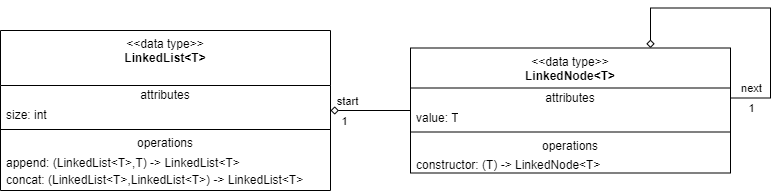
\includegraphics[width=12cm]{linked_list/uml.drawio.png}
\end{center}

A simple standalone type like LinkedList may not be complex enough to showcase the full advantages of UML,
but it is enough to demonstrates the effectiveness of visualization in understanding code.
From the arrows in the image, it is immediately obvious that the start attribute of
LinkedList requires a LinkedNode and LinkedNodes may build off of themselves indefinitely.

UML diagrams are a simple and concise method for conveying the meaning and intention behind a system.
While the syntax is largely standardized, because this language is meant for communication with humans
rather than machines, slight modifications of syntax for the sake of clarity can be made as necessary.
For example, the types of operators may be omitted for an ultra-compact diagram, or kept to ensure an agreement
on the interface implementation is met.

\subsection{Event-B}

Although UML is a powerful tool for communicating the relationship between data types, the visual methodology
falls short when attempting to convey the actionable properties of a system. In continuing the exploration
of modelling languages, we find that the Event-B model not only encompasses actionable system traits, but does
so with consideration of the system's environment. Therefore, Event-B is suitable for formal system analysis
and proving the correctness of software following the model specification.

Data types for Event-B may not exist in the normal sense of the word, but a different approach to data abstraction
through the concepts of machines, contexts, and events is more than suitable for the same purpose:
\begin{itemize}
    \item Machines are somewhat adjacent to classes in OOP, acting like miniature
    programs with some provable traits consisting of variables, invariants, theorems, a single variant, and a list of
    events that may cause the machine to ``run'' (analogous to an object's methods).
    Like class inheritance, new machines can ``refine'' old ones by
    carrying over and adding new entries to the aforementioned traits.
    \item Contexts, on the other hand, are much closer the formal definition of abstract data types,
    defining a set of axioms, theorems, constants and data in the form of carrier sets.
    Contexts can be extended in a similar fashion to class inheritance, with the child context carrying over all properties
    of the parent context.
    \item Finally, events serve as activation conditions for the machine they are assigned to.
    They introduce possibly nondeterministic actions into the system in a formal manner, and must clearly state
    how they affect a machine's variant. A key aspect of events is that all actions within an event are performed simultaneously.
    This means that, unlike in sequential programming languages, the order in which actions are defined have no relevance
    on the outcome of the event. Of course, the restriction of simultaneous execution means that users of the language
    cannot reassign variables in more than one action, nor should they rely on the deterministic nature of normal program execution.
\end{itemize}
All expressions in the above abstractions use formal discrete math notation.

Although a modelling language focused on provable aspects of a system
is not very suitable for a simple low-level data type,
we nonetheless attempt a simplified implementation of \texttt{LinkedList} with only the append method.

\begin{center}
    \fbox{
        \parbox{12cm}{
            LinkedListContext

            \hspace{2em}\textbf{sets}

            \hspace{4em}$Nodes$ // Set of nodes in the list

            \hspace{4em}$References$ // Set of references

            \hspace{2em}\textbf{constants}

            \hspace{4em}$null$ // End of list

            \hspace{2em}\textbf{axioms}

            \hspace{4em}axm1: $References = Nodes \cup \{null\}$

            \hspace{4em}axm2: $\forall n : n \in Nodes \implies n.next \in References$ // All nodes must have a reference

        }
    }
    \fbox{
        \parbox{12cm}{
            AppendEvent

            \hspace{2em}\textbf{any}

            \hspace{4em}$last\_node$

            \hspace{4em}$new\_node$

            \hspace{2em}\textbf{where}

            \hspace{4em}$last\_node \in Nodes$

            \hspace{4em}$\{last\_node\} = \{node \in Nodes : node.next = null \}$ // last\_node is the end of the list

            \hspace{4em}$new\_node.value: T$ // New value must have the same type as existing nodes

            \hspace{4em}$new\_node.next = null$ // New node is end of the list

            \hspace{2em}\textbf{then}

            \hspace{4em}$last\_node.next := new\_node$ // Last node is no longer the last node

            \hspace{4em}$Nodes := Nodes \cup new\_node$ // Add node to list


        }
    }
    \fbox{
        \parbox{12cm}{
            LinkedListMachine

            \hspace{2em}\textbf{variables}

            \hspace{4em}$head$

            \hspace{4em}$value$

            \hspace{4em}$next$

            \hspace{2em}\textbf{invariant}

            \hspace{4em}inv1: $head \in Nodes$

            \hspace{4em}inv2: $value: T$ // Generic type T

            \hspace{4em}inv3: $next \in References$

            \hspace{4em}inv4: $\forall n : n.next \neq null \implies n.next.next \in References$ // Nodes can either end or continue the list

            \hspace{2em}\textbf{events}

            \hspace{4em}AppendEvent

        }
    }
\end{center}

The latest Event-B wiki \cite{eventB} notes future plans to support recursive structured types like inductive LinkedLists
in a more concise format.

% \subsection{SETL} %Maybe? Would need to cite
% \subsection{Bend} %Maybe? Would need to cite
\subsection{Exploration of Conceptual Data Types}

\subsubsection{The Axiomatic Approach to Data Types}

As stated in the introductory textbooks \cite{DTandDS} and \cite{ADTspec}, ADTs at their core are just collections of
data coupled with operations. Both textbooks introduce data types in a manner not unlike the ideas of Event-B,
using formal notation to guarantee precise properties of the given data type. Interestingly, both textbooks
opt to separate data type operations into syntactic and semantic components, where the semantics
contain a list of axioms to be fulfilled by each operation. Note that these axioms are almost entirely removed
from the implementation of the type, acting more as a specification of requirements rather than a how-to guide.

Guaranteed type completeness and correctness are two key features of the axiomatic approach. That is, axioms
encourage operations to consider all possible values that the type may take, especially regarding edge cases and errors.
For example, in our linked list, we need to ensure operations over an empty list are well-defined and that we can
create the empty list itself in the first place. Of course, in the case of linked lists, this is near-trivial,
but focusing on the edge cases in this manner can guarantee correctness of far more complex types.

Consider the axiomatic definition of a linked list, according to the specification of \cite{ADTspec}:
\begin{center}
        \parbox{11cm}{
            NAME

            \hspace{2em}LinkedList(item)

            SETS

            \hspace{2em}$N$: Set of nodes

            \hspace{2em}$I$: Set of items

            SYNTAX

            \hspace{2em}$new: \rightarrow N$

            \hspace{2em}$append: N \times I \rightarrow N$

            \hspace{2em}$concat: N \times N \rightarrow N$

            \hspace{2em}$deleteLast: N \rightarrow N$

            \hspace{2em}$tail: N \rightarrow I$

            \hspace{2em}$isEmpty: N \rightarrow bool$


            SEMANTICS

            $\forall i \in I, \forall n, n1 \in N:$

            \hspace{2em}$deleteLast(append(n, i)) = n$

            \hspace{2em}$tail(append(n, i)) = i$

            \hspace{2em}$tail(concat(n, n1)) = tail(n1)$

            \hspace{2em}$isEmpty(new()) = True$

            \hspace{2em}$isEmpty(append(n, i)) = False$

            \hspace{2em}$tail(new()) = error$ // New initializes a list but does not hold any value

            \hspace{2em}$deleteLast(new()) = error$ // Cannot delete from an empty list

    }
\end{center}

The above axioms do not express the behaviour of each function independently, but instead focus on relationship between one another.
For instance, the axiom $tail(new()) = error$ outlines two properties with one axiom:
\begin{enumerate}
    \item Finding \texttt{tail} on an empty list produces an error.
    \item Since tail produces an empty list error, we must know that \texttt{new} creates an empty list.
\end{enumerate}
Similarly, the axiom $deleteLast(append(n, i)) = n$ shows that append must add the item $i$
to the end of the list $n$, in order for deleteLast to perform correctly.

Unfortunately, this approach may present drawbacks for implementing unknown data types in popular programming languages
\textit{because} of its coupled operation behaviour. In many programming languages, especially non-functional ones,
developers need to implement each data type operation mostly independent of other operations. Therefore, ensuring congruency
between written code and the given specification presents a new challenge for programmers;
data types becoming lost in the translation from dependent specification to independent implementation serve
as an undesirable source of bugs and mistakes. A compiler for such a language would greatly reduce friction between
theory and application, but the semantic expressivity available from the axiomatic approach may be worth the costs.

\subsubsection{A More Constructive Approach}

The textbook \cite{ADTspec} specifies an additional method of data type specification focused on construction
of new objects from old ones. Instead of axioms, each operation can specify relevant pre-conditions and post-conditions.
This method is far closer to the implementation of data types in programming languages, with an uncanny resemblance
to the optional input restrictions seen in Dafny functions. For conciseness, the example given in Section 2.4
serves as a good approximate illustration of the constructive approach outlined in the textbook.

\section{Error Handling and Undefinedness}

Every language explored thus far has found unique methods of breaking down and organizing data for simple use and reuse.
However, the discussion of handling errors and misshapen data is integral to the process of working with types.
After all, if functions have the ability to return any kind of value without warning or due process,
elaborate type systems and proven formal methodology would be meaningless. It seems then, that in order to
maintain the benefits of these type systems, dealing with invalid data is just as vital as working with ideal data.

Nearly every language has its own unique manner of dealing with unexpected data, but for the sake of conciseness,
we only document the two most prevalent methods alongside some honourable mentions. The first and most common
method of handling errors is through the immediate halting of all normal function operations and raising of an exception.
Exceptions propagate all the way through the function stack until it is either caught by a specific construct
or the program terminates. Alternatively, many newer, non-OOP languages instead opt for error handling by value.
Instead of interrupting normal program execution, errors are an integrated data type
that must be handled by calling functions if seen.

\subsection{Throwing Exceptions}

Exceptions are often a integral part of programs that need to deal with failure. Python, for instance, idiomatically
encourages the use of exceptions and try-catch structures to create and contain errors.
Given the flexibility and readability-first approaches to Python scripts, it is entirely understandable that
most programs in Python tend to ask for forgiveness rather than permission, with the expectation that all other parts of
the program will do the same. This means, for better or for worse, that developers do not have to deal with errors
unless they cause a problem at runtime. Often times, and especially outside of documentation,
communication on the kinds of errors a function may raise is virtually non-existent.
Since types were only recently included as part of the language, the most historically effective method of
denoting an error-based value was to use exceptions and force the use of dedicated catch structures.

Interestingly, although Rust primarily encourages handling of errors by value, a subset of errors will allow programs
to panic and act like an exception was thrown. However, the key difference between panics and exceptions
lies in the recoverability: with exceptions, try-catch statements allow the program to recover
from the error and continue execution. On the other hand, panics signal that a program has entered an unrecoverable state.
The execution of all functions stop immediately and the program is terminated.
Panic states are for completely unexpected errors that arise within program execution as opposed to known errors
that may only happen on occasion.

Other languages that use exceptions for error handling are listed below:
\begin{itemize}
    \item TypeScript, as the spiritual successor of JavaScript, inherits JavaScript's
    error handling techniques. Without static types, JavaScript by necessity uses
    dedicated try-catch structures as a means to deal with errors.
    \item APL throws exceptions as most languages would, but the try-catch structure does not lend itself to
    APL's concise and symbolic syntax. Instead, APL offers error guards placed before error-prone code
    to watch for specific kinds of errors and determine recovery actions.
    \item Surprisingly, Haskell's monadic types allow for user-defined exceptions to interrupt the flow of function execution.
    Although this mimics the halting and propagating behaviour of an exception,
    it still remains a part of the expected type system.
\end{itemize}

\subsection{Errors as Values}

Exceptions may be powerful tools for quickly and concisely expressing failures within a code, but they can
easily become overlooked in documentation and program communication, left untouched and unnoticed until runtime.
To better convey the expectation that calling functions should handle the errors created by child calls,
errors as type of value can be used.

Rust's \texttt{Result<T, E>} data type is one of the best examples of treating errors as values.
By breaking down the options for function output into either \texttt{Ok<T>} or \texttt{Err<E>}
types, caller functions know whether they should prepare for the possibility of callee function failure.
Rust will not compile if a possible \texttt{Err} is left unhandled,
so functions must provide a complete path for dealing with both successful values and recoverable errors.
Most of the time, this involves pattern matching on the Ok/Err constructors to get access to the inner value.
However, Rust additionally provides the question mark operator \texttt{?} as a means to concisely propagate errors.
Consider the following code snippet, with three functions: \texttt{error\_prone}, which always returns an error,
\texttt{always\_ok}, which always returns a successful value, and a calling \texttt{middle\_function}
that has a caller itself.
\inputminted{rust}{linked_list/err.rs}
The first statement in \texttt{middle\_function} will contain the integer 0, since the \texttt{?} operator
unwraps result values when they are \texttt{Ok}. Yet, the second statement calls a function that returns an \texttt{Err}.
In this case, the \texttt{?} operator will keep the error-ful value and propagate it to the caller of \texttt{middle\_function}.

The ``update with failure'' operator $(\colon -)$ exists in Dafny for much the same purpose. Upon detecting a failed return value from
a function call, so long as the return type is failure compatible, Dafny will propagate the error to the caller function.
In the event of a success, the value is kept and usable in the rest of the function body as normal.

Similar types to Rust's \texttt{Result} type can be made in any language.
Haskell's \texttt{Either a b} type, for example, is nearly identical, where \texttt{Ok} and \texttt{Err}
are replaced with \texttt{Left a} and \texttt{Right b}.
Even languages without built-in support for inductive types or
errors-by-value can make use of a subset of these concepts. For example,
a Python implementation of Rust's \texttt{Result} type is doable with classes, but loses many of the guarantees
and rule enforcement that stronger typed languages provide:
\inputminted{python}{linked_list/python_result.py}

Much like the benefits of types over regular data, treating errors as a special form of data
promotes the type system to encompass all possible paths a program may take. In turn,
value-errors should result in far more comprehensive code, massively reducing the chance of unexpected runtime errors.

\subsection{Honourable Mention - No Errors, No Problems}

Some languages, like Agda, take an extreme approach to dealing with errors. As a hybrid between a proof assistant
and a regular programming language, Agda virtually eliminates the possibility for errors so long as the usage of
functions is provably correct. The prevention of errors before they can even exist can be a powerful asset
in producing reliable and correct programs, but it also restricts the actions a program can make. For example,
Haskell attempts to live in a functionally pure universe for as long as possible, but recognizes that some
aspects of computing, like IO, will need to be impure for the sake of practicality. Similarly, Agda attempts
to prevent all possible errors from being made, but cannot account for parts of the computer outside its control.
Physical errors, operating system hiccups, and other non-theoretical parts of a computer degrade from an otherwise
perfect program model. Of course, errors of this sort can always be treated as part of the expected data type and
handled according to the previous section.

\section{A Word on Usability}



\section{Conclusion}

Although ADTs are intended primarily for the organization and classification of data (coupled with valid operations),
they enable elegance, correctness, and reliability in almost every other component of programming languages.
From popular OOP languages to user-facing modelling languages, every structuring methodology
brings a new perspective on data and type systems. Even among the 10 programming languages
reviewed in this document, no two forms of manipulating data were quite the same.
As seen in the linked list examples of section 2, every data type may be able to solve the same problem,
but some lenses are clearer than others. Data types and type systems are the backbone of every language,
enabling complex actions through simple abstractions.

\pagebreak
\nocite{*} % keeps all references, even those not referred to
\printbibliography %Prints bibliography

\end{document}